\subsection{Firm Size, Status in Employment, and Formality}
\label{subsec:status-results}

Table~\ref{tab:status-premiums} allows the size profile to differ across
employment relationships. M1, Equation~(\ref{eq:status-size}), estimates a
separate profile for each status in employment while imposing equal size
contrasts for formal and informal workers within that status. M2,
Equation~(\ref{eq:status-size-formality}), also relaxes that restriction.
Both retain the sample, worker controls, and geographic fixed effects used
in M0. Appendix Table~\ref{tab:status-cells} reports the observations
supporting these comparisons.

\begin{table}[htbp]
\centering\small
\caption{Large-firm premiums by status in employment (\%)}
\label{tab:status-premiums}
\begin{tabular}{lrrr}
\toprule
Status in employment & M1 & M2 formal & M2 informal \\
\midrule
\multicolumn{4}{l}{\textit{101+ relative to Solo}} \\
Private-sector employees & 26.0*** & 16.2*** & 16.4*** \\
Government employees & -- & -- & -- \\
Domestic workers & -- & -- & -- \\
Own-account workers & 54.0*** & 53.9*** & 46.2*** \\
Employers & -- & -- & -- \\
Day laborers & 13.0*** & 3.1 & 20.1*** \\
Other workers & 11.9 & 55.5** & 8.1 \\
\midrule
\multicolumn{4}{l}{\textit{101+ relative to 11--19}} \\
Private-sector employees & 10.6*** & 13.1*** & -4.3*** \\
Government employees & 15.5*** & 17.6*** & -23.0 \\
Domestic workers & -- & -- & -- \\
Own-account workers & 19.7*** & 24.4*** & 12.1*** \\
Employers & 49.3*** & 57.5*** & 36.2* \\
Day laborers & 1.6 & 1.7 & 6.8*** \\
Other workers & -19.6 & -- & -24.0 \\
\bottomrule
\end{tabular}
\par\vspace{0.3em}
\begin{minipage}{0.97\textwidth}\footnotesize
Notes: Percentage premiums from M1, Equation~(\ref{eq:status-size}), and M2, Equation~(\ref{eq:status-size-formality}). M1 imposes a common size profile across formality within each employment category. M2 does not. All use 5,426,174 observations. Standard errors are clustered by sector-department. Dashes suppress contrasts with fewer than 30 observations or 10 sector-department clusters at either endpoint, and solo comparisons for government employees and employers. These reporting rules do not remove observations from estimation. * $p<0.10$, ** $p<0.05$, *** $p<0.01$.
\end{minipage}
\end{table}


In M1, the 101+/solo premium is 26.0 percent for private-sector employees
and 54.0 percent for own-account workers. M2 shows that the difference
between these employment categories persists within both formality groups.
Among private-sector employees, the premium is 16.2 percent for formal
workers and 16.4 percent for informal workers. Among own-account workers,
the corresponding estimates are 53.9 and 46.2 percent. All four estimates
are significant with sector-department and sector clustering, as shown in
Appendix Table~\ref{tab:status-clustering}.

The larger informal premium in M0's 101+/solo comparison therefore does
not characterize every employment relationship. M2 does not reject equal
formal and informal 101+/solo log-wage contrasts within private-sector
employment ($p=0.944$) or own-account work ($p=0.296$), using
sector-department clustering. The own-account contrast exceeds the
private-employee contrast within each formality group under both clustering
procedures. These comparisons concern differences between size premiums,
not differences in wage levels between formal and informal workers.

Figure~\ref{fig:status-formality-premiums} reports the complete M2 size
profiles for private-sector employees and own-account workers. Similar
101+/solo estimates within a group do not imply identical formal and
informal profiles at intermediate sizes. Relative to 11--19 workers, formal
private-sector employees in 101+ firms earn 13.1 percent more, whereas
informal private-sector employees earn 4.3 percent less. The latter contrast
has $p=0.055$ with sector clustering. Among own-account workers, the
101+/11--19 premium is 24.4 percent for formal workers and 12.1 percent for
informal workers. The informal contrast is significant with
sector-department clustering but not with sector clustering ($p=0.073$).

\begin{figure}[htbp]
  \centering
  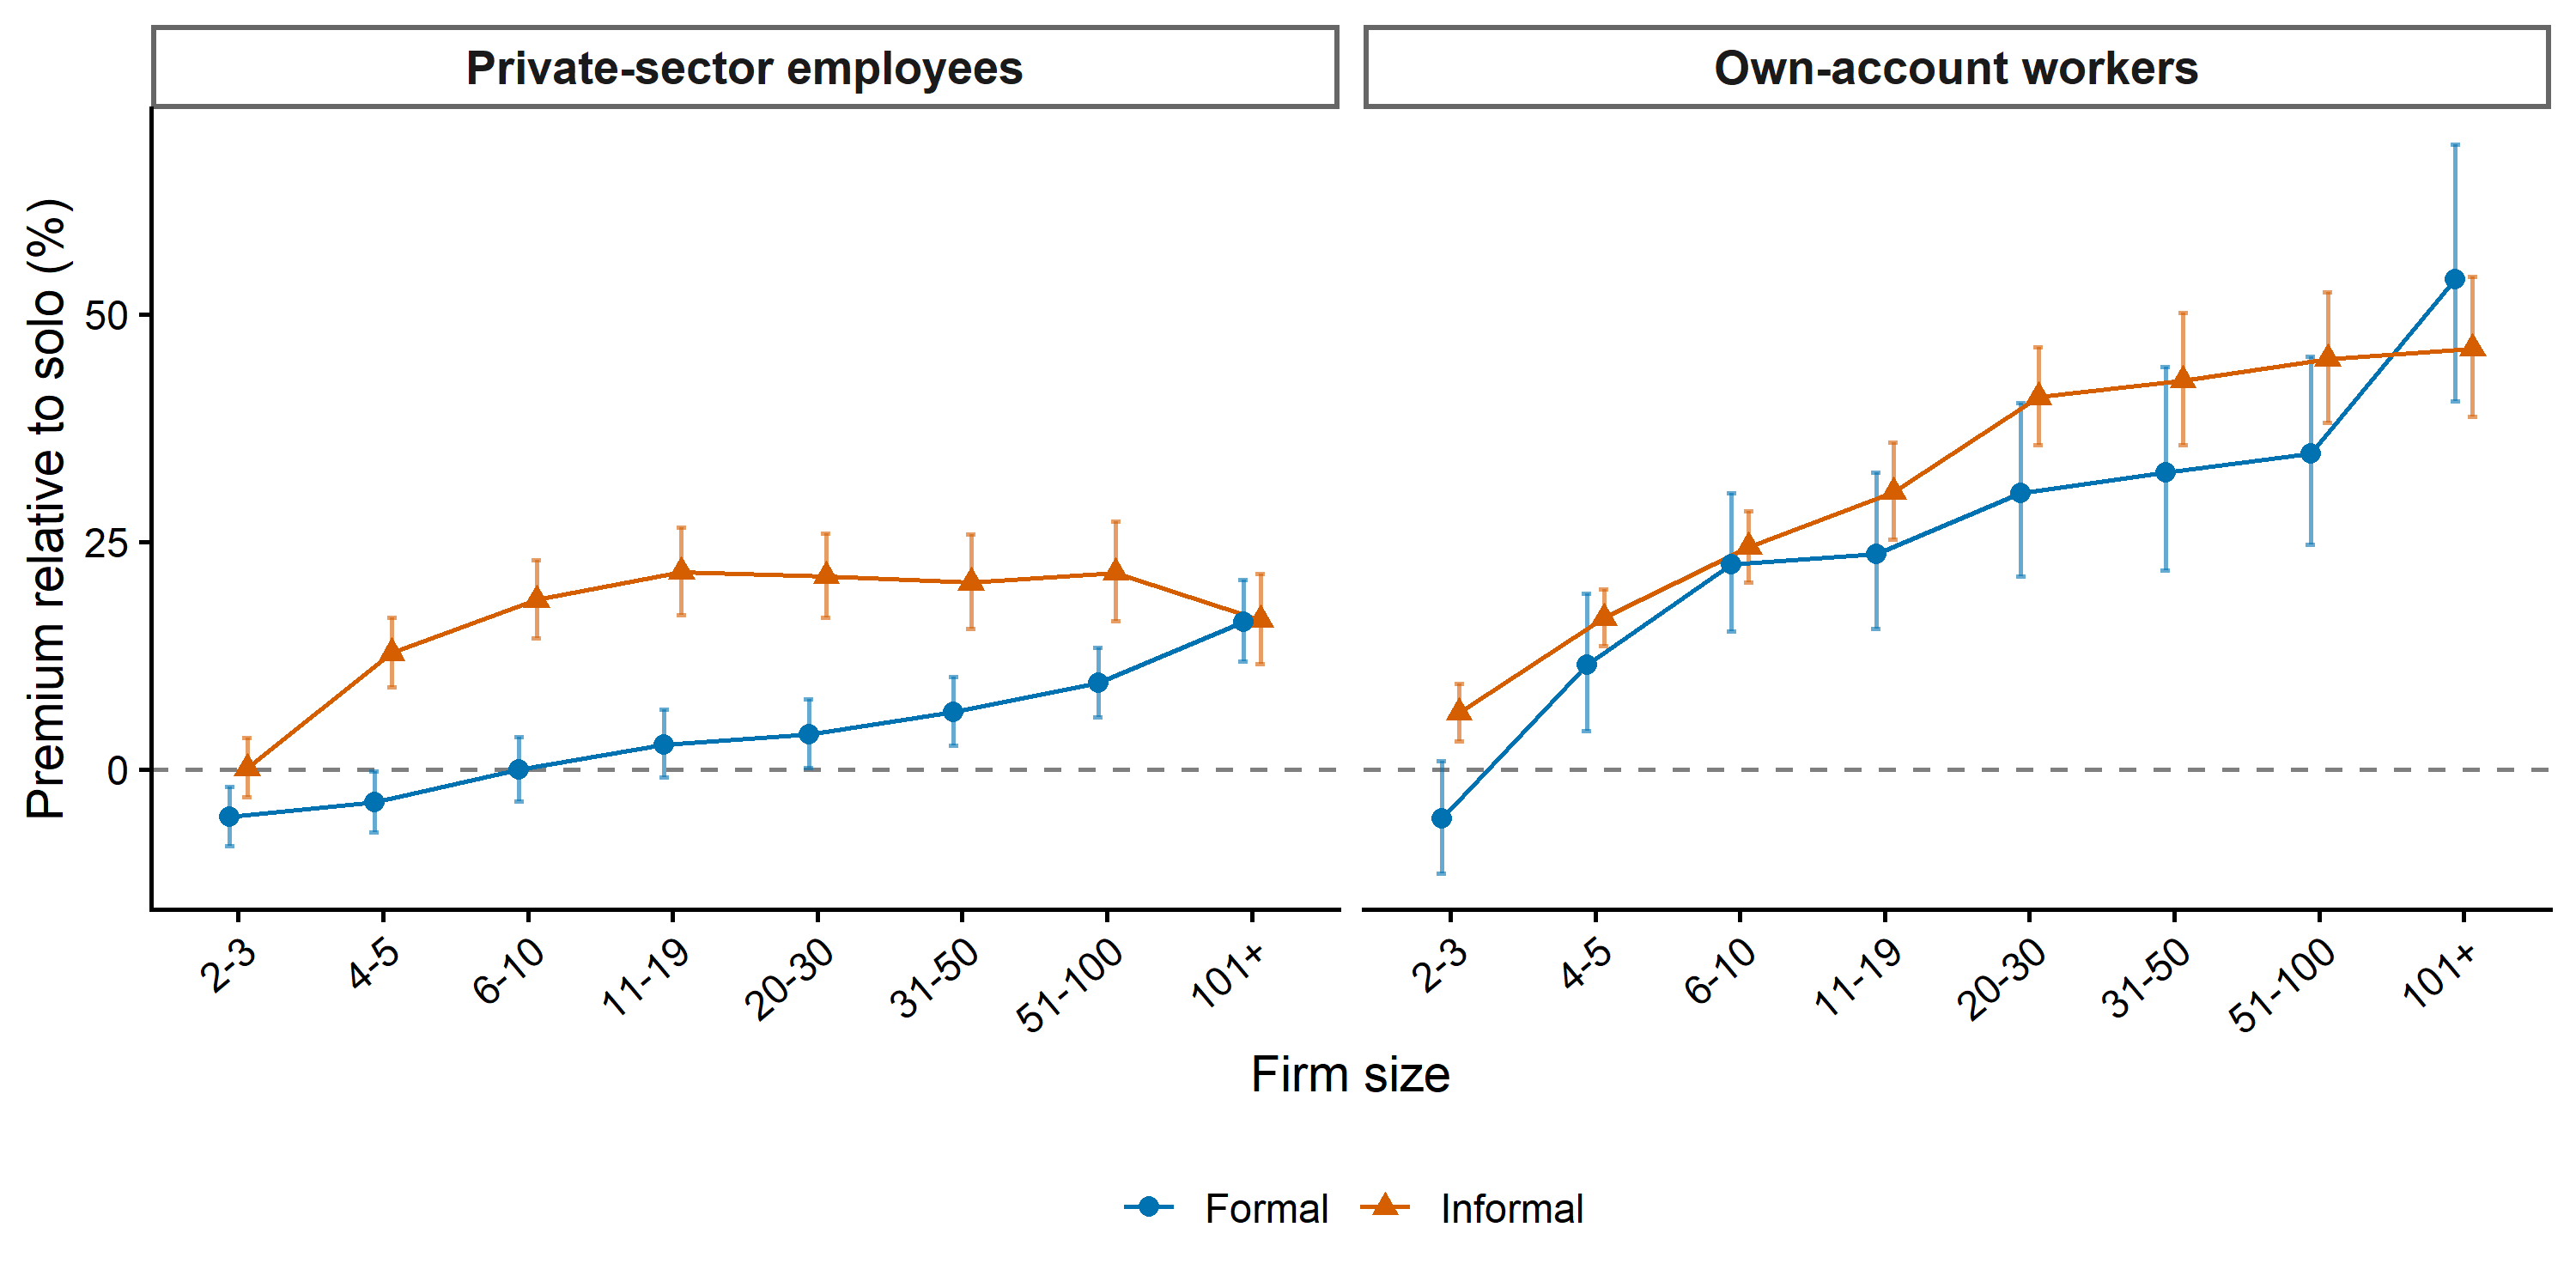
\includegraphics[width=\textwidth]{status_formality_premiums_en.png}
  \caption{M2 firm-size premiums within employment and formality groups}
  \label{fig:status-formality-premiums}
  \begin{minipage}{0.97\textwidth}\footnotesize
  Notes: Reference workers have the same status in employment and formality
  and report solo work. Bars are 95 percent confidence intervals using
  sector-department clustering.
  \end{minipage}
\end{figure}

For government employees and employers, 11--19 workers is more informative
than solo work as a reference. The data contain only 18 government employees
and 507 employers reporting solo work, classifications that warrant checking
against the questionnaire instructions. We retain these records in estimation
but do not interpret their solo contrasts. Relative to formal workers in
11--19 units, the M2 formal 101+ premium is 17.6 percent for government
employees and 57.5 percent for employers. Estimates for some other groups
are imprecise. For example, only 27 domestic-worker observations report
101+ across the full period. The two unpaid family observations and the
absence of unpaid workers from other households do not permit size comparisons
for those categories.

Appendix Tables~\ref{tab:status-profiles-solo} and
\ref{tab:status-profiles-11-19} report the full M1 and M2 profiles under
both reference categories. Figure~\ref{fig:status-other-profiles} shows
the supported comparisons for government employees, employers, domestic
workers, and day laborers. These differences across employment relationships
qualify the comparison with \citet{BalkanTumen2016}. M0 resembles their
finding of a larger informal premium, but M2 does not establish that ranking
within each status in employment.
\FloatBarrier
